\section{Data Handling}\label{subsec:Scaling}
\subsection{Scaling}
The distribution of values for different features can vary immensely, and for most 
cost functions, this is a problem. For some features, a deviation on the magnitude 
of $10^3$ can be a good approximation, whereas for others it can be a vast 
overestimation. When a model is to define which direction it wants to tune, it is 
crucial that the errors across all features are weighted equally. Scaling aims levitate 
this problem by transforming all features to have a relatively equal range of values while
simultaneously preserving all information regarding each feature. The choice of how one 
chooses to scale the data will heavily affect the performance of the model and is therefore
a part of the model. 
\\
\subsubsection{Standard Scaler}
The \emph{Standrad Scaler} implemented in this rapport uses Scikit-learns's \emph{StandardScaler}
\cite{StandardScaler}. The standard scaler function scales each feature individually by subtracting 
the mean and dividing by the standard deviation. In doing so the resulting scaled data has a mean 
of 0 and a standard deviation of 1. Mathematically the standard scaler, $\mathcal{S}$ transforms 
a dataset $\x$ as 
\begin{align}
    \mathcal{S} \left(\x\right) = \frac{\x - \boldsymbol{\mu} _x}{\boldsymbol{\sigma}_x} ,
\end{align}
where $\boldsymbol{\mu} _x$ and $\boldsymbol{\sigma}_x$ are vectors with the elements being 
the mean and standard deviation respectively for each feature.

\subsection{Principal Component Analysis}
\begin{figure}
    \centering
    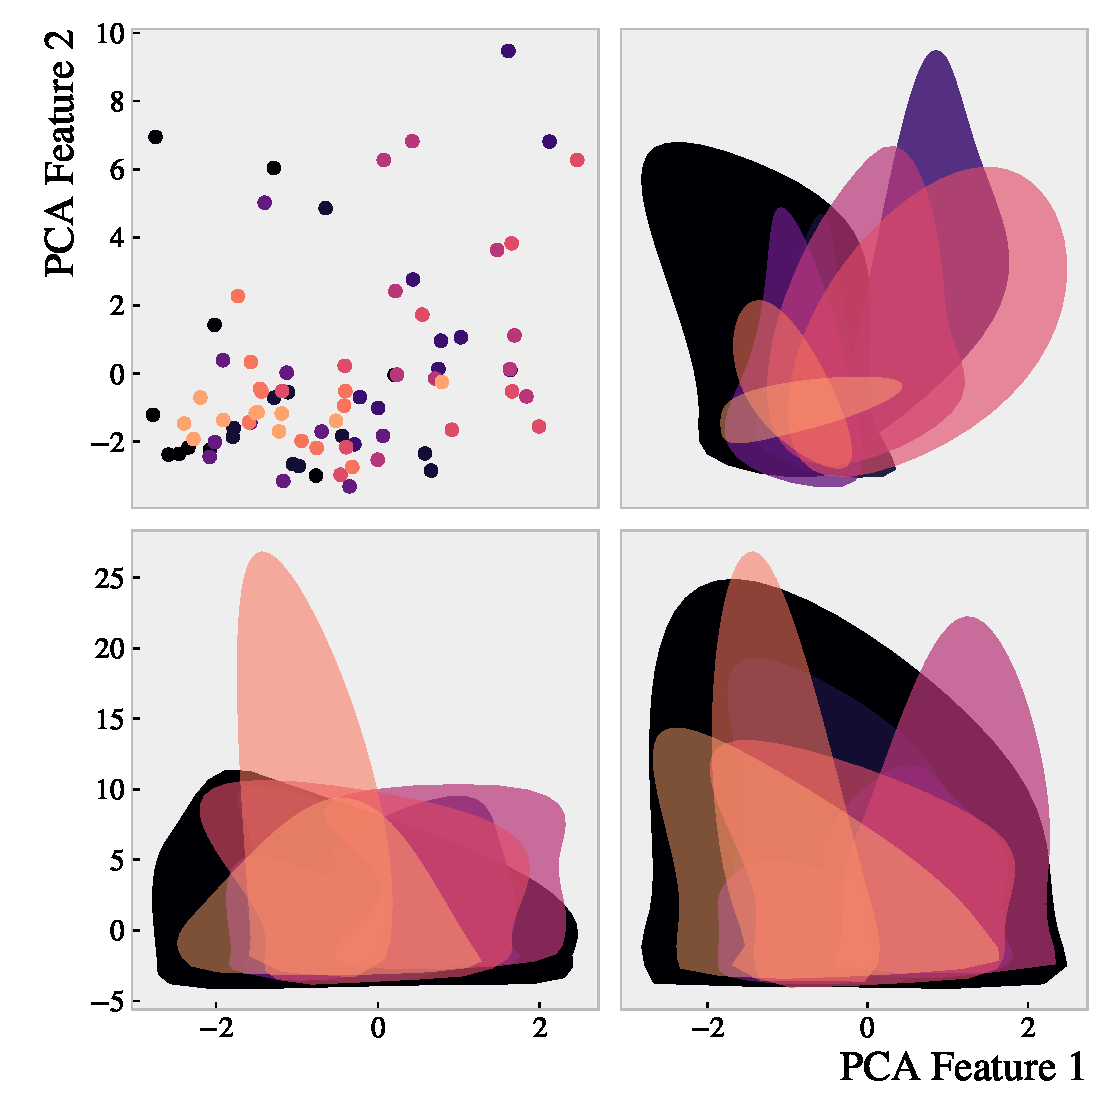
\includegraphics[width=0.6\textwidth]{Figures/MLResults/DataHandling/PCA/PCAPlotFirst.pdf}
    \caption{The distribution of the two PCA-features containing most variation for (left to right, 
    up to down) 10, 10, 100 and 500 samples from each channel. Each sample filling the requirement 
    with being less than one standard deviation from the mean of both features, respectively.}
    \label{fig:PCA1}
\end{figure}
\begin{figure}
    \centering
    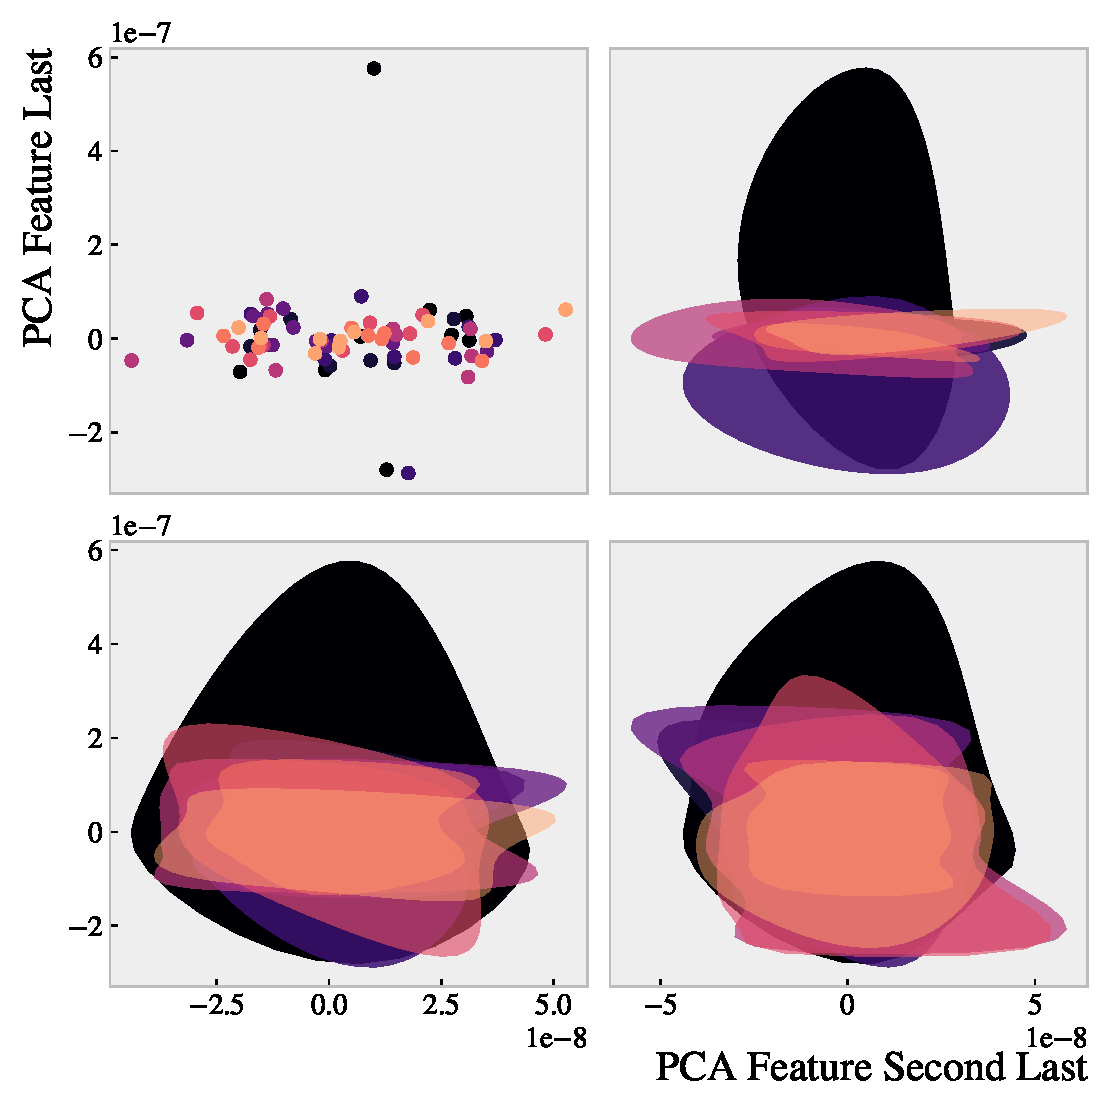
\includegraphics[width=0.6\textwidth]{Figures/MLResults/DataHandling/PCA/PCAPlotLast.pdf}
    \caption{The distribution of the two PCA-features containing the least amount of variation for (left to right, 
    up to down) 10, 10, 100 and 500 samples from each channel. Each sample filling the requirement 
    with being less than one standard deviation from the mean of both features, respectively.}
    \label{fig:PCA2}
\end{figure}


